\documentclass[12pt]{article}
\usepackage{graphicx} % Required for inserting images
\usepackage[spanish]{babel}
\usepackage{lmodern}
\renewcommand{\familydefault}{\sfdefault}
\usepackage{geometry}
\usepackage{setspace}
\usepackage{float}
\usepackage{xcolor}
\usepackage{amsmath}
\usepackage{tikz}
% Solo una vez se carga hyperref, con tus opciones y el linkcolor
\usepackage[colorlinks=true, urlcolor=blue, linkcolor=black]{hyperref}

\begin{document}
\definecolor{azul}{RGB}{0, 168, 255}
\definecolor{azul2}{RGB}{7, 74, 163}

\begin{titlepage}
    \thispagestyle{empty}
    \newgeometry{left=2cm, right=1cm, top=2cm, bottom=2cm}
    
    % Gráfico de fondo corregido para ser fiable
    \begin{tikzpicture}[overlay, remember picture, fill opacity=0.7]
        \begin{scope}[shift={(current page.center)}]
            \rotatebox{-45}{\fill[azul2] (5, -15) rectangle (12, 15);}
            \rotatebox{-45}{\fill[azul] (3, -15) rectangle (5, 15);}
        \end{scope}
    \end{tikzpicture}
    
    \begin{spacing}{1.5}
        {\Huge \bfseries \noindent PRÁCTICA 3}
        \vspace{10pt}

        {\LARGE PERMANENCIA DE DATOS CON UNA BASE DE DATOS}
        
        \vspace{1cm}
        
        {\Large Equipo:} \\
        {\Large Beltrán Saucedo Axel Alejandro} \\
        {\Large Cerón Samperio Lizeth Montserrat} \\
        {\Large Higuera Pineda Angel Abraham} \\
        {\Large Lorenzo Silva Abad Rey} \\
        {\Large 4BV1.}
    \end{spacing}
    
    \vspace{1.5cm}

    \begin{minipage}{7.5cm} % Ancho ajustado
        {\Large ESCUELA SUPERIOR DE CÓMPUTO}
    \end{minipage}

    \vfill % Empuja el contenido hacia el final de la página

    \begin{flushleft}
        {\Large \color{black}
        % Comando \textbf corregido con llaves
        \textbf{TECNOLOGÍAS PARA EL DESARROLLO DE APLICACIONES WEB}}
        
        \vspace{0.5cm}
        
        13/10/2025
    \end{flushleft}
    \vspace{1cm}
\end{titlepage}

\newpage
\tableofcontents
\newpage

\section{Introducción}
\subsection*{Planteamiento del problema}
El problema que se aborda es la falta de persistencia de datos en la aplicación.
La aplicación guarda los datos en la memoria mientras está funcionando, pero se pierde al reiniciar la aplicación.
Se necesita una solución que garantice lo siguiente:
\begin{itemize}
    \item La información de cada item se almacena de forma permanente.
    \item Los usuarios pueden recuperar, actualizar o eliminar estos items en cualquier momento.
    \item La aplicación mantenga un registro organizado y estructurado de todos los paquetes.
\end{itemize}

\subsection*{Propuesta de solución}
La solución propuesta es el desarrollo de una API RESTful utilizando FastAPI para la lógica de negocio y SQLModel para la gestión de la base de datos , permitiendo así la persistencia de datos.
Componentes clave de la solución:
\begin{itemize}
    \item \textbf{Framework Web (FastAPI):} Se utiliza para construir la interfaz de la API, definiendo las rutas (URLs) que permitirán a los usuarios interactuar con la información de los paquetes. Un framework web moderno y rápido para construir APIs con Python 3.7+ basado en estándares como OpenAPI y JSON Schema.
    \item \textbf{SQLModel:} Se emplea para definir la estructura de la información (qué es un "ítem", qué campos tiene, y cuál es su identificador único).
    \item \textbf{Base de datos SQLite:} Se utiliza un motor de base de datos SQLite (database.db) para almacenar los datos en un archivo físico. De esta manera, la información perdura aunque la aplicación se detenga o se reinicie.
    \item \textbf{SQLModel Engine y Session:} Se configura un motor de conexión (engine) y un sistema de sesiones (SessionDep) para establecer una comunicación eficiente y segura entre la aplicación y el archivo de la base de datos.
\end{itemize}

\section{Fundamentos Teóricos}

Para la correcta creacion de nuestra práctica, es importante que entendamos las relaciones entre las tecnologías y los conceptos que ya revisados para la creación de una API, esta vez implementando persistencia de datos.

\subsection*{API RESTful}
Una API RESTful es un estilo de arquitectura para diseñar aplicaciones en red. Se basa en un conjunto de principios que utilizan los métodos estándar de HTTP para realizar operaciones sobre los recursos. Cada recurso. que aqui seran items, es identificable a través de una URL única. Este enfoque simplifica la comunicación entre el cliente y el servidor.\cite{ref1}

\subsection*{Entorno de Trabajo y Herramientas Principales}
\begin{itemize}
    \item \textbf{Python:} Es el lenguaje de programación sobre el que se construye toda la lógica de la aplicación. Su sencilla sintaxis y su amplia cantidad de librerías lo hacen ideal para el desarrollo web.\cite{ref2}
    \item \textbf{FastAPI:} Framework web moderno para construir APIs con Python. Sus características más destacadas son la rapidez, la validación de datos automática mediante Pydantic y la generación de documentación interactiva , que fue crucial para probar los endpoints de nuestra API.
    \item \textbf{Uvicorn:} Es un servidor ASGI ultrarrápido, utilizado para ejecutar la aplicación FastAPI. Permite que la API maneje múltiples peticiones de forma asíncrona, mejorando el rendimiento.\cite{ref3}
\end{itemize}

\subsection*{Persistencia de Datos}
La persistencia de datos es la capacidad de un sistema para poder conservar la información posterior de la duración de una sola ejecución. En nuestra practica pasada, los datos eran volátiles, ya que se almacenaban en una lista en memoria. En esta práctica, se implementa la persistencia a través de los siguientes componentes:

\begin{itemize}
    \item \textbf{SQLite:} Es un motor de base de datos relacional, autocontenido y que no requiere un servidor. Almacena toda la base de datos en un único archivo (en nuestro caso, \texttt{database.db}). Es ideal para desarrollo y aplicaciones de pequeña a mediana escala por su simplicidad y portabilidad.
    
    \item \textbf{SQLAlchemy:} Es una librería que funciona como un Mapeador Objeto-Relacional (ORM). Un ORM es una técnica que actúa como un "traductor" entre el código orientado a objetos y las tablas de una base de datos relacional. Permite manipular la base de datos utilizando código Python en lugar de escribir consultas SQL directamente.
    
    \item \textbf{SQLModel:} Es una librería que combina \textbf{SQLAlchemy} y \textbf{Pydantic}, creada por el mismo autor de FastAPI. Permite definir la estructura de los datos, las validaciones y el esquema de la base de datos en una sola clase, reduciendo la duplicación de código y simplificando el desarrollo. En nuestra práctica, las clases como \texttt{Item} son modelos de SQLModel que representan tanto la tabla en la base de datos como los datos que la API recibe y envía.\cite{ref4}
\end{itemize}

\section{Diagrama UML}
\begin{figure}[H]
    \centering
    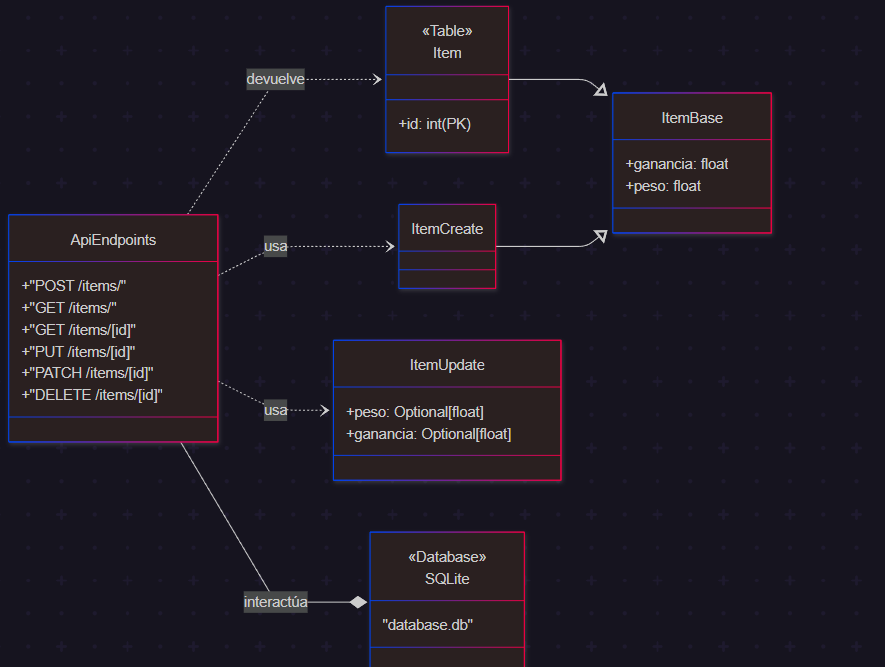
\includegraphics[width=1\textwidth]{Imagenes/Diagrama.png}
\end{figure}


\section{Implementación}
\subsection*{Código:}
En esta seccion tendremos los nuevos modulos que usamos para el funcionamiento de la practica.\\

Debemos entender la diferencia entre esta practica y la anterior, ya que pueden parecer iguales, pero tienen una diferencia crucial. 
En la practica anterior, nuestra API gestionaba los datos de los items en una lista en memoria, lo cual tenia una principal desventaja,
que al reiniciar nuestro servidor, todos los datos se perdian. 
En cambio, esta vez integramos una base de datos para asegurar la permanencia de los datos.

\begin{figure}[H]
    \centering
    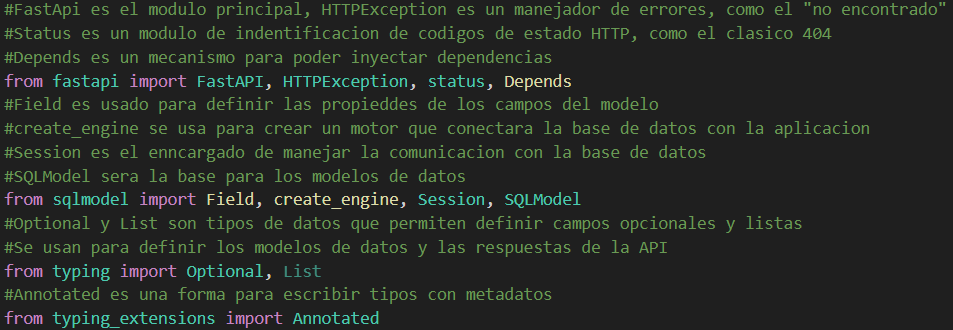
\includegraphics[width=1\textwidth]{Imagenes/Imagen WEB 3_1.png}
\end{figure}

El principal cambio que podemos ver aqui es la adicion de la libreria SQLModel, la cual nos permitira interactuar con la base de datos,
gracias a sus capacidades provenientes de SQLAlchemy y Pydantic.

\begin{figure}[h!]
    \centering
    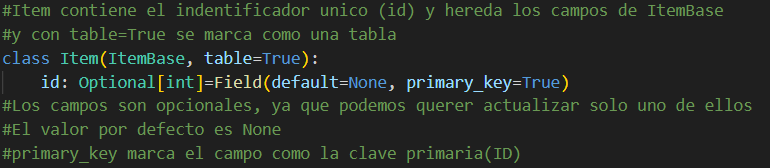
\includegraphics[width=1\textwidth]{Imagenes/Imagen WEB 3_2.png}
\end{figure}

En esta parte, podemos ver que los modelos de datos fueron redefinidos usando SQLModel y asi poder mapearlos en una tabla en nuestra base de datos.
Se agrego 'table=true', que le indica a SQLModel que la clase esta representando una tabla en la base.
Otro cambio es en id, que ahora lo definimos como la clave primaria de nuestra tabla. Esto hara que la base de datos se encargue de ir generando los id's
de forma automatica.\\

\begin{figure}[H]
    \centering
    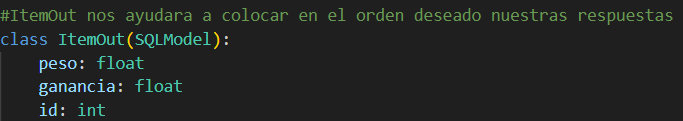
\includegraphics[width=1\textwidth]{Imagenes/Imagen WEB 3_3.png}
\end{figure}

Esta funcion tiene el unico proposito de mostrarnos los datos en el orden deseado, el cual es peso/ganancia/id, ya que originalmente los mostraba en desorden.

\begin{figure}[h!]
    \centering
    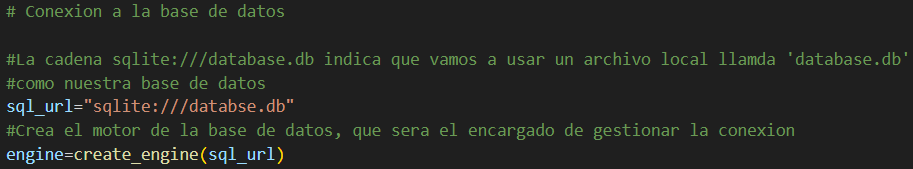
\includegraphics[width=1\textwidth]{Imagenes/Imagen WEB 3_4.png}
\end{figure}

Aqui tenemos la nueva adicion mas importante, la cual se encargara de la configuracion y manejo de la conexion con la base de datos (que estara en SQLite).
Esta sera almacenada en un archivo bajo el nombre de database.db.
Tambien tenemos lo que vendria a ser nuestro 'motor', por decirlo de una forma, que funcionara como el centro de comunicaciones entre la API y nuestro database.db

\begin{figure}[h!]
    \centering
    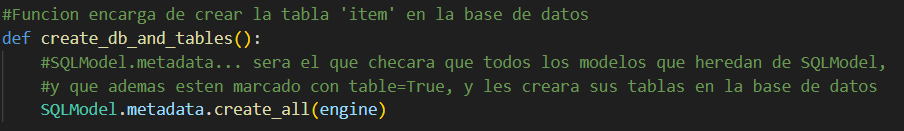
\includegraphics[width=1\textwidth]{Imagenes/Imagen WEB 3_5.png}
\end{figure}

Esta funcion sera la encargada de la creacion de las tablas y solo se ejecutara una vez al iniciar la aplicacion.
Crea las tablas correspondientes en la base si es que no existen.

\begin{figure}[H]
    \centering
    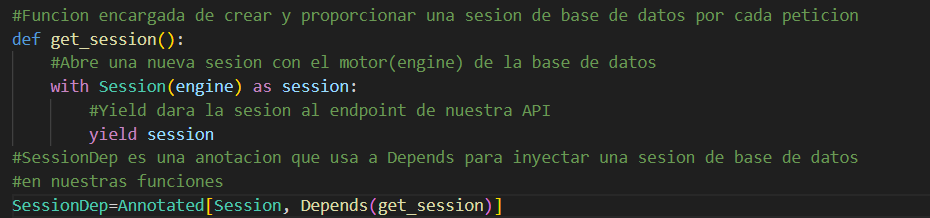
\includegraphics[width=1\textwidth]{Imagenes/Imagen WEB 3_6.png}
\end{figure}

Aqui implementamos un sistema de sesiones por peticion. Esto se refiere a que cada vez que la API recibe una solicitud, una nueva sesion de comunicacion con la base de datos
se abre, y esta misma se cierra en automatico al terminar la solicitud, lo cual nos garantiza un manejo seguro de las conexiones.

\begin{figure}[H]
    \centering
    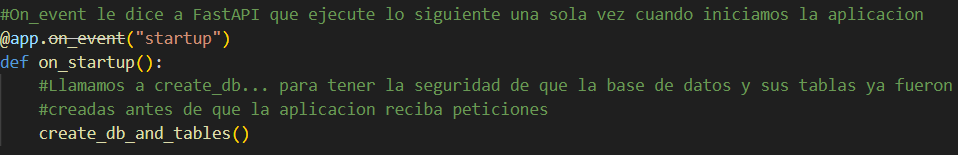
\includegraphics[width=1\textwidth]{Imagenes/Imagen WEB 3_7.png}
\end{figure}

Este evento se ejecuta en el instante en el momento en que la API se termine de iniciar,antes de que cualquier usuario mande una peticion y solo se ejecuta una vez.
Y esto no garantiza que la base de datos y sus tablas ya existan antes de que los usuarios empiezen a mandar peticiones.

\newpage % Opcional, para que las referencias empiecen en una página nueva

% Añade la línea "Referencias" al índice como si fuera una sección
\addcontentsline{toc}{section}{Referencias}
\begin{thebibliography}{99}

    \bibitem{ref1} IBM. (s.f.). ¿Qué es una API REST? Recuperado el 14 de octubre de 2025, de \url{https://www.ibm.com/mx-es/topics/rest-apis}
    \bibitem{ref2} Python Software Foundation. (s.f.). Acerca de Python™. Resumen Ejecutivo. Recuperado el 14 de octubre de 2025, de \url{https://www.python.org/doc/essays/blurb-es/}
    \bibitem{ref3} Ramírez, S. (s.f.). FastAPI. Recuperado el 14 de octubre de 2025, de \url{https://fastapi.tiangolo.com/es/}
    \bibitem{ref4} Ramírez, S. (s.f.). SQLModel. Recuperado el 14 de octubre de 2025, de \url{https://sqlmodel.tiangolo.com/es/}

\end{thebibliography}

\end{document}